\chapter{Examples of System Operator Met Measurement Requirements}\label{ch:requiremenexamples}

%collection of a few examples and reference or establish a table that compares some of the requirements of some of the major system operators in North America and Europe (and maybe elsewhere if we can find the info)?

\section{Comparison of Requirements in various jurisdictions}

\begin{itemize}
    \item \textbf{AESO}: Alberta Electric System Operator in Calgary, Alberta, Canada [AESO,2011]
    \item \textbf{CAISO}: California Independent System Operator [CAISO, 2014, 2016]
    \item \textbf{BPA}: Bonneville Power Administration in Portland, Oregon, USA [BPA, 2015]
    \item \textbf{ERCOT}: Electricity Council of Texas in Austin, Texas, USA [ERCOT, 2012]
    \item \textbf{NYISO}: New York Independent System Operator in Rensselaer,NY,USA [NYISO, 2016] 
    \item \textbf{PJM}: Independent System Operator in Audubon, PA, USA [PJM, 2016]
    \item \textbf{HECO}: Hawaiian Electric Company, Maoui, Hawaii [HECO, 2016]
    \item \textbf{LitGrid}: in Vilnius, Lithuania [LiTGRID, 2010]
\end{itemize}


\section{Met Measurement Example from Califorina Independent System Operator in USA}

The following tables are examples from the California Independent System Operator taken from the Appendix Q of their \textit{Eligible Intermittent Resources Protocol} (EIRP) from December 2020. 

\begin{figure}[h!]
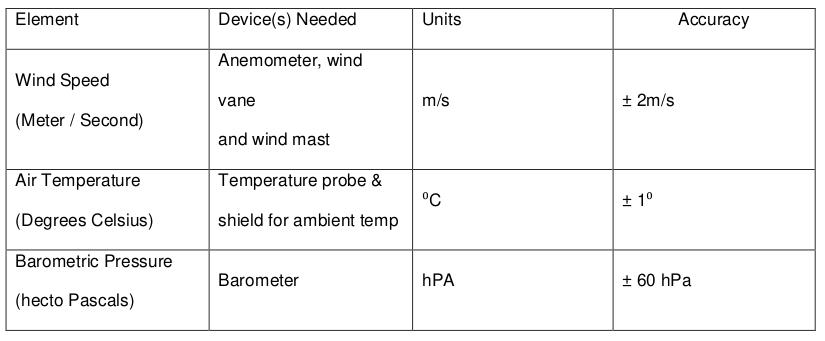
\includegraphics[width=0.75\textwidth]{figures/CAISO_tableQ1.png}
\caption{\textit{Wind Eligible Intermittent Resources Telemetry Data Points}} 
\label{fig:CAISO_tableQ1}
\end{figure}

\begin{figure}[h!]
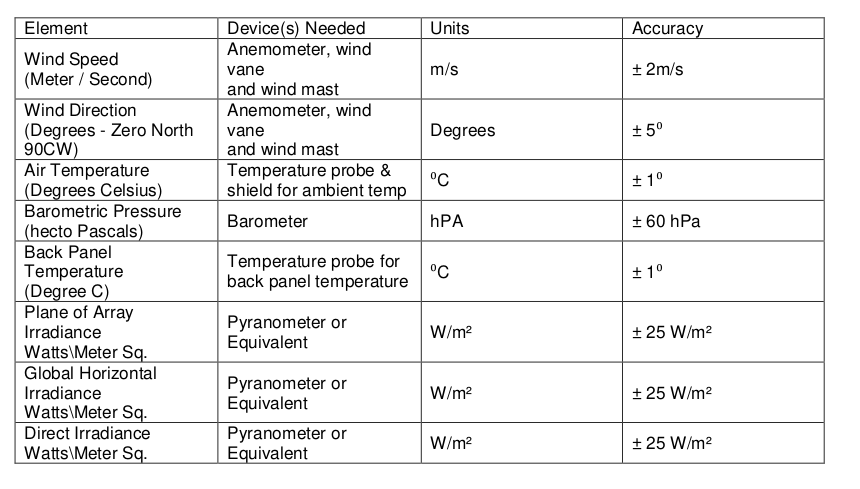
\includegraphics[width=0.75\textwidth]{figures/CAISO_tableQ3.png}
\caption{\textit{Solar Eligible Intermittent Resources Telemetry Data Points}} 
\label{fig:CAISO_tableQ3}
\end{figure}


\section{Met Measurement Example from Irish System Operator EIRGRID Group}

Examples from the Met Data Requirement document of the Irish transmission system operator EIRGRID, which is part of the grid code for wind generation units  under section WFPS 1.7.1.6: \\

\textbf{Time Delays and Data Quality}\\
Digital signal changes from the Controllable WFPS shall be relayed to the TSO
Telecommunication Interface Cabinet within 1 second of the associated change of
state event. Analogue signal changes shall be relayed within 5 seconds and with an error
of 0.5\% or less, with the exception of the Meteorological Data required as per PPM
1.7.1.2.1, which shall be updated within 5 seconds and with an error of 2.5\% or less.


\textbf{System accuracies and Measurement resolution}\\
The meteorological data signals provided shall be as detailed in Table 1: Meteorological data signal
accuracy and resolution and Table 2: Meteorological data variable and their error threshold limit. The WFPS shall provide an updated signal every 1 minute.

\begin{figure}[h!]
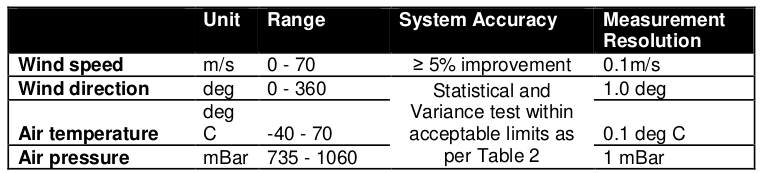
\includegraphics[width=0.75\textwidth]{figures/EIRGRID_table1.png}
\caption{\textit{Meteorological data signal accuracy and resolution}} 
\label{fig:EIRGRID_table1}
\end{figure}

\begin{figure}[h!]
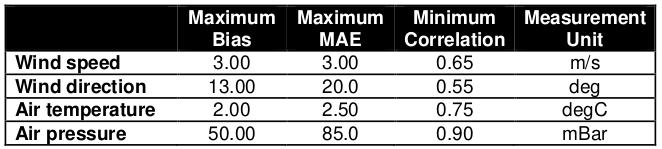
\includegraphics[width=0.75\textwidth]{figures/EIRGRID_table2.png}
\caption{\textit{Meteorological data variable and their error threshold limit for statistical tests}} 
\label{fig:EIRGRID_table2}
\end{figure}


%\section{Met Measurement Example from Alberta Electric System Operator in Canada}